% Physical Review E submission source (single author, revised 2026-07-31).
% Claim boundaries checked against repository artifacts on 2026-07-19.
% Detailed derivations and secondary numerical families are in
% encounter_modality_supplement.tex, which compiles without this file's .aux.
\documentclass[aps,pre,reprint,amsmath,amssymb,longbibliography,floatfix]{revtex4-2}

\usepackage{cmap}
\usepackage[T1]{fontenc}
\usepackage{lmodern}
\usepackage{graphicx}
\usepackage{bm}
\usepackage{booktabs}
\usepackage{hyperref}
\hypersetup{
  hidelinks,
  pdftitle={Spectral diagnostics and local fixed-budget sensitivity of critical points in finite encounter-reaction models},
  pdfauthor={Xiaoxiao Zhouyi},
  pdfsubject={Finite-model encounter-reaction modality under spatially redistributed reactivity},
  pdfkeywords={encounter reaction, reaction-time density, Doi model, Green operator, modality fold, fixed-budget sensitivity}
}
\usepackage{placeins}

\graphicspath{{../artifacts/figures/}{./figures/}{./}}
\renewcommand{\topfraction}{0.92}
\renewcommand{\textfraction}{0.05}
\renewcommand{\floatpagefraction}{0.82}

\newcommand{\dd}{\mathrm d}
\newcommand{\e}{\mathrm e}
\newcommand{\Tgen}{\mathcal T}
\newcommand{\Lfree}{\mathcal L_0}
\newcommand{\Rfree}{\mathcal R_0}
\newcommand{\Gres}{\mathcal G}

\begin{document}

\title{Spectral diagnostics and local fixed-budget sensitivity of critical points in finite encounter-reaction models}

\author{Xiaoxiao Zhouyi}
\email{xiaoxiao.zhouyi@bristol.ac.uk}
\affiliation{School of Engineering Mathematics and Technology, University of Bristol,
Bristol BS8 1TW, United Kingdom}

\date{July 31, 2026}

\begin{abstract}
Reaction-time densities of confined encounter reactions can contain several
transport-generated time windows, yet whether those windows appear as
critical points of the measured flux depends jointly on transport, the
initial law, and the spatial reaction field. We develop an exact finite-model
calculus for diagnosing and steering those critical points. First, a
reaction-support Green reduction separates free transport from volume
killing. Second, the generalized Descartes rule gives a necessary spectral
gate: a reversible finite-model density with \(m\) interior modes requires at
least \(2m-1\) sign changes in its ordered nonzero residues. Third, an exact
Fr\'echet--Duhamel derivative gives the response of the critical-point
equation to every killing rate, and projection onto the tangent space of a
declared reactivity budget identifies the locally steepest feasible
redistribution in a chosen metric.

Two families of finite generators exercise the calculus. Direct
matrix-exponential derivatives locate a nondegenerate reaction-density fold
in a finite two-reactant continuous-time Markov chain under a rate-ratio
control, and independent continuation recovers the generic \(1/2\)
critical-point-separation and \(3/2\) prominence exponents of the fold
normal form. A separate finite-radius two-dimensional family redistributes
reactivity at an exactly fixed per-grid killing sum and exhibits the same
nondegenerate fold structure and exponents on three grids. The critical
controls of the two-dimensional family are grid- and budget-measure
sensitive and are reported as finite-generator mechanism certificates. An
exact fold-transfer theory, a cell-averaged refinement ladder run under two
independent transport discretizations, and a \(2\times10^7\)-walker
lattice-free Brownian realization then settle the continuum question: the
physical matched-budget path carries no interior continuum fold; the
finite-grid critical controls are coarse-discretization artifacts, and the
organizing fold is extrapolated to the admissibility edge of the family,
where the far-channel rate vanishes. The fold-transfer proof, the refinement-ladder roots, and detailed
endpoint, coordinate, clock, capacity, and multichannel audits are
reported in the Supplemental Material.
\end{abstract}

\maketitle

\section{Introduction}
\label{sec:introduction}

The reaction time of two mobile particles can retain information that a mean
reaction time or a single long-time decay rate suppresses. In confinement,
first contact need not be reaction: encounter can be imperfect and
reaction can be restricted to selected spatial regions. The measured density
then depends jointly on transport, encounter geometry, and the reaction
observable. Multiple critical points of the density---time-stationary points in the
sense of singularity theory, not critical phenomena---can reflect
dynamically distinct
reaction streams, but their existence does not by itself identify which
mechanism produced them.

Multimodal passage and reaction-time laws have established transport,
geometric, internal-state, and encounter-history mechanisms. Confined
encounter laws, exact propagators, heterogeneous transmission sites,
multi-target reductions, and transport-generated multiple peaks are developed
in Refs.~\cite{levot2020firstencounter,levot2022firstencounter,
giuggioli2013encounter,giuggioli2020exact,
giuggioliSarvaharman2022transmission,sarvaharmanGiuggioli2023particle,
sarvaharmanGiuggioli2020biased,marrisGiuggioli2024persistent,
giuggioliEtAl2024multitarget}. Imperfect reaction has likewise been treated
through Doi volume killing, radiation boundaries, and heterogeneous
reactivity \cite{doi1976stochastic,isaacson2009rdme,
isaacsonMauroNewby2016uniform,chapmanErbanIsaacson2016reactive,
grebenkov2019spectral,grebenkov2020sphericaltraps}. Static killing fields and
partially reactive network elements have already been rearranged at fixed
total strength, and position-dependent Robin reactivity has been optimized
under an integral constraint
\cite{nguyenGrebenkov2010porous,scottEtAl2021tubular,
nicolaouMulder2023flux}. Besga \emph{et al.} previously established a Brownian
first-passage shape transition in which a finite-time maximum--minimum pair
merges under a target-distance/initial-spread control
\cite{besgaEtAl2021dynamical}. We therefore do not claim either the fold
criterion \(f_t=f_{tt}=0\), a two-clock shape transition, or any of the other
ingredients above as new.

The narrower problem here is differential. Suppose a finite killed generator
has a reaction-density fold, so that
\(f_t=f_{tt}=0\) at positive time. Can one (i) determine whether its observable
spectrum has enough sign variation to permit the requested number of modes,
(ii) compute the response of the fold equation to a spatial killing
redistribution, and (iii) identify the most effective infinitesimal
redistribution compatible with a fixed budget? We answer those questions
exactly for declared finite generators, then test the resulting calculus in a
finite encounter chain and a finite-radius two-dimensional family.

The distinction between a \emph{strict extremum} and a
classifier-\emph{resolved mode} is important. The main article uses
derivative-certified folds only. Endpoint morphology, synchronous-clock
controls, catalytic-coordinate sensitivity, finite-grid trimodality,
capacity calibration, and generalized-inverse-Gaussian (GIG) screening are
preserved as secondary audits in the standalone Supplemental Material
\cite{supplementalMaterial}. Those calculations delimit the causal language
but are not needed to establish the two fold certificates presented here.

The seven main claims and their boundaries are summarized in
Table~\ref{tab:evidence}; a transfer theory, a cell-averaged refinement
ladder, and an off-lattice realization (Sec.~\ref{sec:bridge}) settle what
the finite certificates do and do not imply in the continuum. Figure~\ref{fig:model-fold} shows the spatial
channel picture and the generic fold geometry.

\begin{table*}[!t]
\caption{\label{tab:evidence}
Evidence hierarchy used in the main article.}
\begin{ruledtabular}
\begin{tabular}{p{0.25\textwidth}p{0.27\textwidth}p{0.39\textwidth}}
Statement & Evidence & Boundary\\
\hline
Reaction-support Green reduction
& Exact conditional operator identity and finite Woodbury specialization
& Volume killing on a declared support; no unqualified Robin trace identity or
continuum meromorphic continuation\\
Finite reversible spectral gate
& Generalized-Descartes corollary and primary-generator reconstruction
& Necessary, not sufficient; not a channel-rank bound and not applied to
complex-spectrum, Jordan, or continuum laws\\
Fixed-budget modality susceptibility
& Exact finite Fr\'echet--Duhamel identity, projected optimum, and independent
directional checks
& Infinitesimal interior-rate design in a declared budget and metric; no
finite-amplitude, binary-mask, moving-support, or continuum optimum\\
Finite encounter-chain fold
& Direct finite-matrix derivatives, root solve, residuals, transversality, and
independent normal-form scaling
& One finite model; minority-channel splitting probability
\(8.95\times10^{-6}\)\\
Finite-radius 2D matched-budget folds
& Three finite-generator folds, independent normal-form scaling, and a second
budget-measure check
& Critical controls are nonmonotone and budget-sensitive; no converged
continuum critical control\\
Fold-transfer theory
& Exact transfer statements with Supplemental Material proof
& Sectorial and jet hypotheses instantiated numerically, not proved for
these schemes\\
Continuum bridge (negative result)
& Cell-averaged two-discretization ladder to \(33^2\) nodes;
\(2\times10^7\)-walker off-lattice realization
& Negative result for this geometry only; sectorial and jet hypotheses
instantiated numerically; five sampled off-lattice controls; extrapolants
are estimates with the cross-scheme gap reported alongside\\
\end{tabular}
\end{ruledtabular}
\end{table*}

\begin{figure*}[!t]
\centering
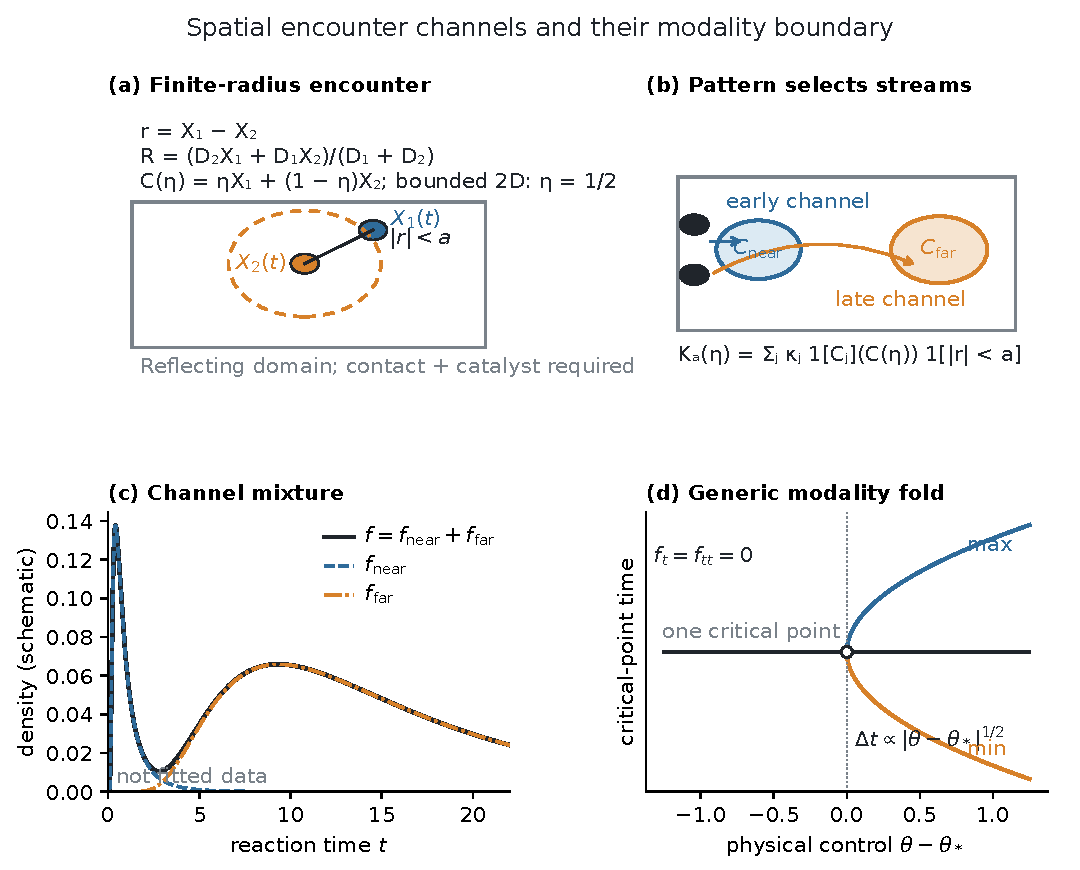
\includegraphics[width=6.65in]{encounter_model_and_fold}
\caption{\label{fig:model-fold}
Spatial encounter channels and their modality boundary. (a) Reaction requires
finite-radius contact and catalytic activation at a declared affine encounter
location. (b) Separated patches select early and late streams. (c) Their sum
can be bimodal; the curves are schematic and are not fitted data. (d) At a
generic fold, a maximum--minimum pair is created with square-root separation
under a physical control.}
\end{figure*}

\section{Finite encounter model and Green reduction}
\label{sec:green}

Let \(X_i(t)\in\Omega\subset\mathbb R^d\) be two independent particles before
reaction, with generator \(\Lfree\) and reflecting outer boundaries. A finite
contact radius \(a>0\) and an affine catalytic coordinate
\[
C_\eta(x_1,x_2)=\eta x_1+(1-\eta)x_2,\qquad 0\leq\eta\leq1,
\]
define channel killing fields
\begin{align}
K_{a,j}^{(\eta)}
&=\kappa_j(C_\eta)\mathbf 1_{C_j}(C_\eta)
\mathbf 1_{\{|x_1-x_2|<a\}},\notag\\
K_a^{(\eta)}&=\sum_jK_{a,j}^{(\eta)}.
\label{eq:doi-killing}
\end{align}
The unreacted joint density obeys
\begin{equation}
\partial_t p=\Lfree p-K_a^{(\eta)}p.
\label{eq:joint-fp}
\end{equation}
With \(S(t)=\int p\) and
\(f_j(t)=\int K_{a,j}^{(\eta)}p\), reflecting boundaries give the exact mass
balance
\begin{equation}
-S'(t)=f(t)=\sum_j f_j(t).
\label{eq:mass-balance}
\end{equation}
The catalyst coordinate is part of the physical model: the midpoint and the
diffusion-decoupling weighted centre are unequal when the particle
diffusivities differ. Coordinate algebra, the transformed domain, Doi--Robin
qualifications, and the finite-grid midpoint audit are given in the
Supplemental Material \cite{supplementalMaterial}.

Write the volume killing operator on
\(\mathsf H=L^2(\mathcal D)\) as
\begin{equation}
V=\Gamma^*\mathsf K\Gamma,\qquad
\Tgen=\Lfree-V,
\label{eq:killed-operator}
\end{equation}
where \(\Gamma\) restricts a function to the reaction support,
\(\Gamma^*\) extends it by zero, and \(\mathsf K\) is a bounded nonnegative
multiplication operator on that support. It may have a kernel. For
\({\rm Re}\,s\) above the spectral bound, define
\begin{equation}
\Rfree(s)=(s-\Lfree)^{-1},\qquad
\Gres(s)=\Gamma\Rfree(s)\Gamma^*.
\label{eq:restricted-green}
\end{equation}
Whenever the displayed inverse exists, the inverse-free resolvent identity is
\begin{equation}
(s-\Tgen)^{-1}
=\Rfree-\Rfree\Gamma^*\mathsf K
 (I+\Gres\mathsf K)^{-1}\Gamma\Rfree.
\label{eq:woodbury-operator}
\end{equation}
Thus, for \(u=\Gamma\Rfree q_0\), the restricted state and transformed
reaction density are
\begin{equation}
x=(I+\Gres\mathsf K)^{-1}u,\qquad
y=\mathsf K(I+\Gres\mathsf K)^{-1}u.
\label{eq:support-density}
\end{equation}
No inverse of \(\mathsf K\) is required. This separation exposes free
transport through \(\Gres\), geometry through \(\Gamma\), and intrinsic
chemistry through \(\mathsf K\).

For a finite continuous-time Markov chain (CTMC), adopt row vectors. Let
\(L_0=L_1\oplus L_2\), let columns of \(U\) select reactive states, and let
\(K\) be diagonal in channel rates. Then
\begin{equation}
T=L_0-UKU^\mathsf T,\qquad
f_j(t)=\alpha\e^{Tt}UKe_j.
\label{eq:finite-channel}
\end{equation}
The finite support matrix
\[
G(s)=U^\mathsf T(sI-L_0)^{-1}U
\]
gives
\[
\det(sI-T)=\det(sI-L_0)\det[I+G(s)K].
\]
The second determinant locates only candidate killed poles coupled to the
reaction support. Dark transport modes, numerator cancellation, and
observable residues must still be checked. Splitting probabilities are
computed from the stable killed solve
\begin{equation}
\bm\pi=\alpha(-T)^{-1}UK,
\label{eq:splitting-killed}
\end{equation}
when the reachable live chain is transient. Exact time derivatives are
\begin{equation}
\partial_t^n f(t)=\alpha\e^{Tt}T^nUK\bm1.
\label{eq:time-derivatives}
\end{equation}
The detailed two-site exclusion test model and zero-frequency diagnostics are
reported in the Supplemental Material \cite{supplementalMaterial}.

\section{Spectral gate and fixed-budget susceptibility}
\label{sec:modality-design}

\subsection{A necessary sign-variation condition}
\label{sec:spectral-bound}

Consider a finite killed model whose observable density has a real,
diagonalizable spectral expansion. After equal decay rates are grouped and
zero residues removed, write
\begin{equation}
f(t)=\sum_{j=1}^{n}a_j\e^{-\lambda_jt},
\qquad 0<\lambda_1<\cdots<\lambda_n.
\label{eq:spectral-density}
\end{equation}
Reversibility is a sufficient hypothesis because detailed balance makes the
killed generator similar to a real symmetric matrix. Applying the classical
generalized Descartes rule \cite{jameson2006descartes} to
\begin{equation}
f_t(t)=-\sum_{j=1}^{n}\lambda_ja_j\e^{-\lambda_jt}
\label{eq:spectral-derivative}
\end{equation}
after \(x=\e^{-t}\) gives the following corollary:
\[
\#\{\hbox{positive-time zeros of }f_t\}
\leq V(a_1,\ldots,a_n),
\]
where zeros are counted with multiplicity and \(V\) is the number of ordered
residue sign changes. Hence \(m\) nondegenerate interior maxima separated by
minima require
\begin{equation}
V(a_1,\ldots,a_n)\geq2m-1.
\label{eq:spectral-mode-bound}
\end{equation}
This is a necessary falsification gate, not a mode-count predictor. Three
sign changes can coexist with only one positive critical point, and a
rank-one killing support can already produce a bimodal phase-type density.
Reaction-support rank therefore cannot replace the observable residues.

Full symmetric eigendecompositions rebuild the two primary generators used in
the numerical audits. Reversibility, the gate's hypothesis, is verified
directly for both free generators: every live transition is two-way, a
spanning-tree reconstruction of the detailed-balance log-weights closes on
all off-tree edges with maximum cycle inconsistency \(2.4\times10^{-14}\)
(961 states) and \(9.1\times10^{-14}\) (2025 states), and the recovered
measure symmetrizes the killed generator. Equal decay rates are grouped at a
relative tolerance \(2\times10^{-10}\) before residues are summed; at that
tolerance no two eigenvalues of either generator merge. The 961-state finite
encounter generator is evaluated
at its three reported critical points; the separate 2025-state
three-channel generator is evaluated at five detected critical
points. Across the four relative residue cutoffs \(10^{-12}\), \(10^{-10}\),
\(10^{-8}\), and \(10^{-6}\) (relative to the summed absolute grouped
residues), the
minimum retained sign counts are 444 and 191, respectively, above the
necessary bounds three and five. Because these reconstructions reuse the
same generator constructors and critical-time artifacts, they test decomposition
and reconstruction rather than discover roots independently. Full cutoff,
counterexample, and reconstruction details are in the Supplemental Material
\cite{supplementalMaterial}.

\subsection{Budget-projected modality response}
\label{sec:budget-gradient}

For a finite live-state transport generator \(L\), let
\begin{equation}
T(k)=L-\operatorname{diag}k,\qquad
f(t;k)=\alpha\e^{T(k)t}k,
\label{eq:killing-design-model}
\end{equation}
where \(k>0\) on the allowed design support. For
\(k_\epsilon=k+\epsilon h\), put \(H=-\operatorname{diag}h\). The exact
Fr\'echet--Duhamel identity is
\begin{equation}
D\e^{Tt}[H]=\int_0^t\e^{T(t-s)}H\e^{Ts}\,\dd s
\label{eq:design-duhamel}
\end{equation}
\cite{alMohyHigham2009frechet}. Since
\(f_t=\alpha\e^{Tt}Tk\), its complete directional derivative is
\begin{equation}
D_kf_t(t;k)[h]
=\alpha D\e^{Tt}[H]Tk+\alpha\e^{Tt}(Hk+Th).
\label{eq:modality-susceptibility}
\end{equation}
The second term is essential because the killing field is also the measured
reaction observable. Writing this linear functional as \(g^\mathsf Th\),
\begin{equation}
g_i=(\alpha\e^{Tt}T)_i-k_i(\alpha\e^{Tt})_i
-\int_0^t(\alpha\e^{T(t-s)})_i(\e^{Ts}Tk)_i\,\dd s.
\label{eq:modality-gradient}
\end{equation}

Let \(c>0\) define the declared budget \(c^\mathsf Th=0\), and let
\(M\succ0\) define the local norm \(h^\mathsf TMh=1\). Put
\begin{equation}
\lambda_B=\frac{c^\mathsf TM^{-1}g}{c^\mathsf TM^{-1}c},
\qquad \widetilde g=g-\lambda_Bc.
\label{eq:budget-projection}
\end{equation}
Cauchy--Schwarz on the budget tangent space gives
\begin{equation}
h_*=\frac{M^{-1}\widetilde g}
{\sqrt{\widetilde g^\mathsf TM^{-1}\widetilde g}},
\qquad
\max D_kf_t[h]=\sqrt{\widetilde g^\mathsf TM^{-1}\widetilde g}.
\label{eq:optimal-redistribution}
\end{equation}
At a double stationary point, \(\widetilde g\ne0\) means that some
infinitesimal feasible redistribution is transverse to the fold. The
direction depends on the selected budget \(c\) and metric \(M\); it is not a
coordinate-free global optimum.

An eleven-state test model, with seeded random positive diagonal metric
\(M\) and budget vector \(c\) (uniform draws on \([0.65,1.85]\) and
\([0.55,1.65]\)), compares Eq.~\eqref{eq:modality-gradient} with a
basis Fr\'echet calculation, 256 independently generated budget-zero finite differences, a
state permutation, and 20,000 random feasible directions. The relative
Duhamel error is \(3.3\times10^{-15}\), the maximum independent finite-difference
error is \(2.4\times10^{-8}\), and the best random response is \(0.933\) of
Eq.~\eqref{eq:optimal-redistribution}. At the finite encounter fold below,
the chain-rule reconstruction of the computed log-rate transversality agrees
to \(6.8\times10^{-15}\) relative error. The orthogonal near-to-far
fixed-state-sum redistribution has nonzero transversality
\(-1.1621\times10^{-5}\).

\section{Physical folds in finite encounter generators}
\label{sec:fold-results}

At a fold of density critical points under a physical parameter \(\theta\),
\begin{equation}
f_t(t_*,\theta_*)=f_{tt}(t_*,\theta_*)=0.
\label{eq:physical-fold}
\end{equation}
The generic nondegeneracy conditions are
\begin{equation}
a_*=f_{t\theta}(t_*,\theta_*)\ne0,\qquad
b_*=f_{ttt}(t_*,\theta_*)\ne0.
\label{eq:fold-nondegenerate}
\end{equation}
Taylor expansion gives
\[
f_t=a_*\Delta\theta+\frac{b_*}{2}\Delta t^2+
o(|\Delta\theta|+|\Delta t|^2).
\]
On the side where \(-2a_*\Delta\theta/b_*>0\), the new maximum and minimum
separate as
\begin{equation}
\Delta t_\pm=
\pm\sqrt{-\frac{2a_*}{b_*}\Delta\theta}
+o(|\Delta\theta|^{1/2}),
\label{eq:fold-roots}
\end{equation}
and integrating the quadratic derivative gives prominence proportional to
\(|\Delta\theta|^{3/2}\). These equations concern a physical control that can
change both channel weights and shapes; a freely adjusted mixture weight is
not substituted for \(\theta\).

\subsection{Finite two-reactant CTMC certificate}
\label{sec:finite-ctmc}

The finite encounter chain has sites \(0,\ldots,30\). Its two independently
clocked walkers have interior total (attempt) jump rates \(0.7\) and \(0.2\),
respectively, and a common right bias \(0.3\). Their interior left/right rates
are therefore
\((0.245,0.455)\) and \((0.07,0.13)\). At a boundary an out-of-range jump is
omitted, giving the declared reflecting (holding) convention. If \(L_1\) and
\(L_2\) are the corresponding row generators, the free pair generator is the
Kronecker sum \(L_1\oplus L_2=L_1\otimes I+I\otimes L_2\), and the initial law
is concentrated at \((3,15)\). Killing acts only at the reactive co-locations
\((13,13)\) and \((30,30)\), with rates \(\kappa_{\rm near}\) and
\(\kappa_{\rm far}\), respectively. Transport and the initial law remain
fixed. We set \(\kappa_{\rm far}=-\log 0.4=0.9162907319\) and vary
\begin{equation}
\theta=\log(\kappa_{\rm near}/\kappa_{\rm far}),
\label{eq:ctmc-control}
\end{equation}
so that \(\kappa_{\rm near}=\kappa_{\rm far}e^\theta\). Parameter derivatives
are computed by propagating the column state and its sensitivity,
\begin{equation}
p'=T^\mathsf Tp,\qquad
s'=T^\mathsf Ts+T_\theta^\mathsf Tp,\qquad s(0)=0,
\label{eq:augmented-sensitivity}
\end{equation}
in one augmented matrix exponential; all semigroup actions are sparse
matrix-exponential actions in IEEE double precision. Time derivatives use
Eq.~\eqref{eq:time-derivatives}; no sampled-curve maximum is used to locate
the fold, which is obtained by a Powell hybrid root solve on the scaled
residual pair \((f_t,f_{tt})\) with parameter tolerance \(10^{-11}\) and
guarded acceptance thresholds.

The numerical root is
\begin{equation}
t_*=37.0749586402,\qquad
\theta_*=-9.6753635853,
\label{eq:ctmc-fold-point}
\end{equation}
corresponding to
\(\kappa_{\rm near}=5.755410148\times10^{-5}\). Residuals and margins are
made dimensionless with the fold time and density:
\(|f_t|t_*/f=7.1\times10^{-15}\),
\(|f_{tt}|t_*^2/f=6.8\times10^{-13}\), third derivative
\(f_{ttt}t_*^3/f=69.94\), and parameter transversality
\(f_{t\theta}t_*/f=-0.1962\). Independent continuation uses a symmetric
geometric ladder of fourteen control offsets
\(\Delta\theta=\pm0.001\)--\(0.064\) that play no role in locating the
fold; the log--log fits use the six two-peak-side offsets
\(\Delta\theta\le0.032\) and give slopes \(0.50095\) for separation and
\(1.50877\) for prominence, while the seven one-peak-side offsets confirm
the absence of any critical pair (Fig.~\ref{fig:gigfold}). The normal-form
amplitude is tested as well: the predicted separation
\(2\sqrt{-2a_*/b_*}\,\Delta\theta^{1/2}=5.554\,\Delta\theta^{1/2}\)
matches the measured separations to \(0.01\%\) at \(\Delta\theta=0.001\)
and \(0.7\%\) at \(\Delta\theta=0.064\). Mass closure is \(4.0\times10^{-15}\), and survival
at \(t=5000\) is \(1.3\times10^{-21}\).

\begin{figure*}[!t]
\centering
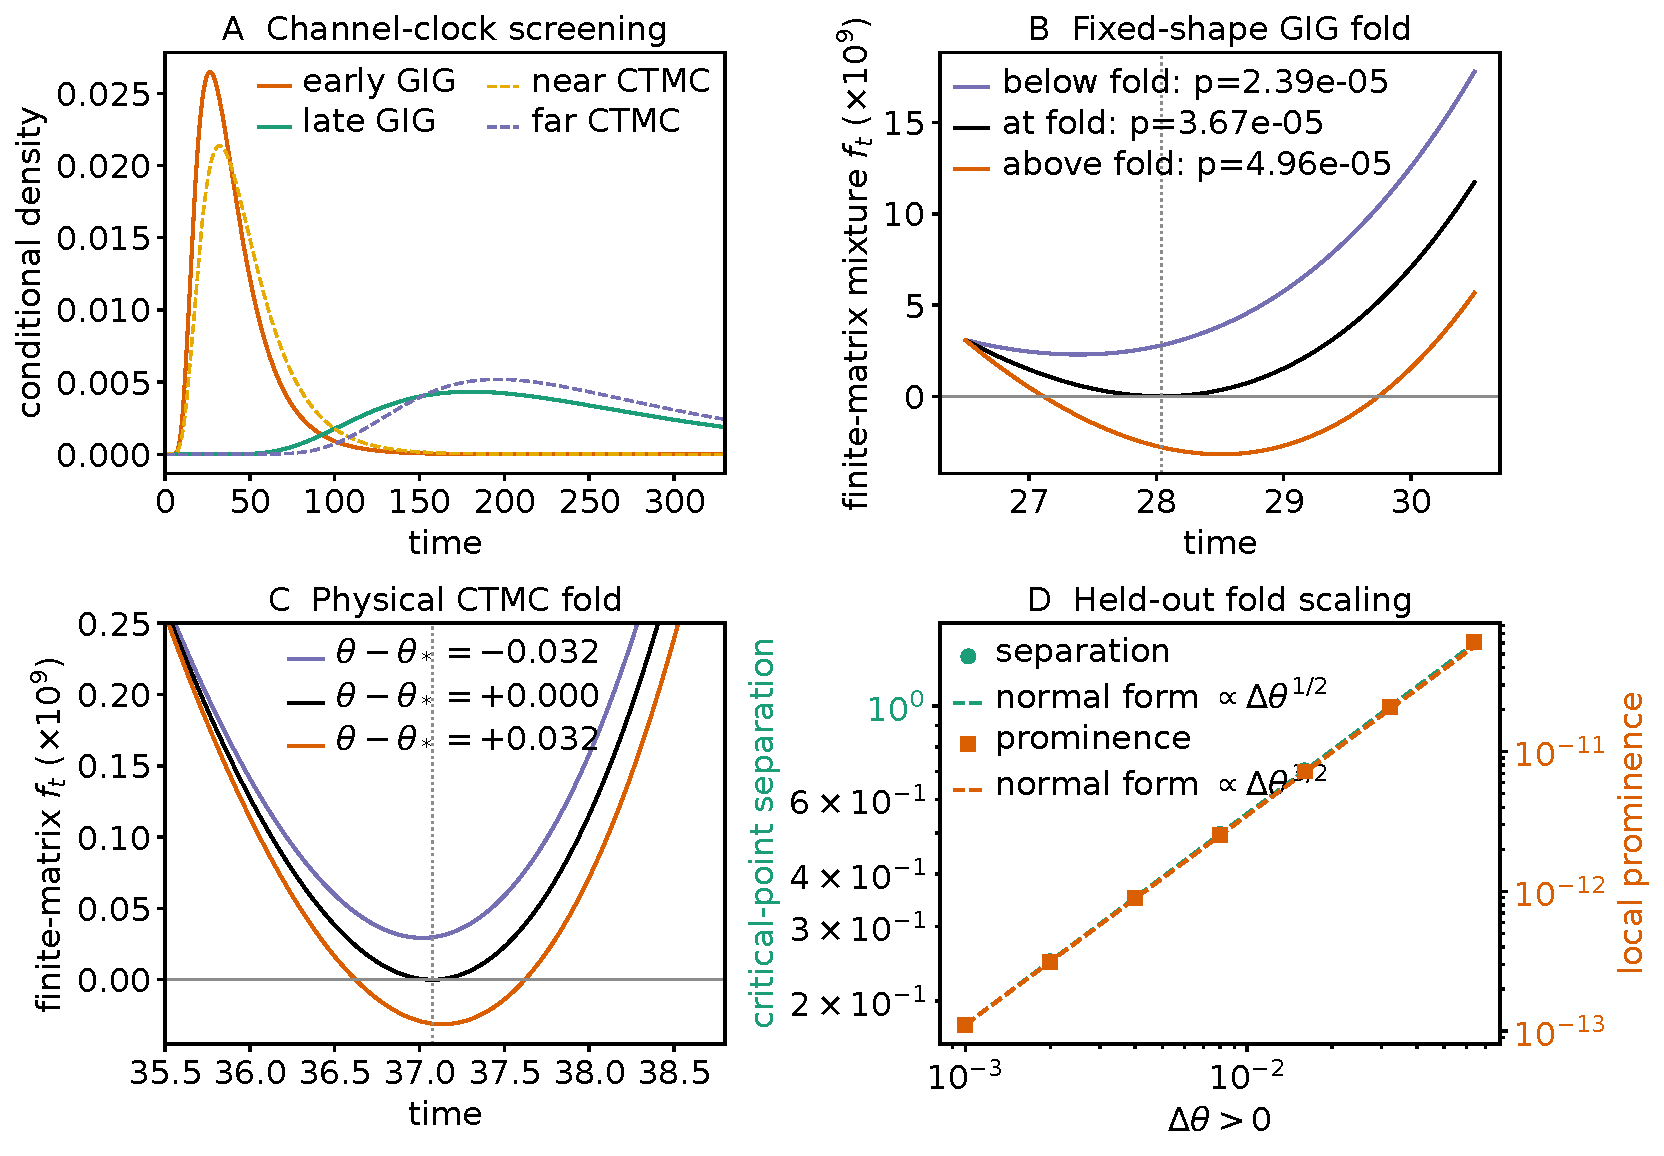
\includegraphics[width=6.65in]{gig_fold_validation}
\caption{\label{fig:gigfold}
Finite-CTMC fold certificate. The fold is located directly from
matrix-exponential derivatives of the killed generator. Independent continuation
recovers the \(1/2\) separation and \(3/2\) prominence exponents. The
free-space GIG channel clocks shown in the figure are screening estimates,
not replacements for the finite-matrix calculation; their derivation and
clock-control audits are in the Supplemental Material
\cite{supplementalMaterial}. The near-channel splitting probability at the
fold is \(8.95\times10^{-6}\), so the result establishes a mechanism rather
than two comparably observable streams.}
\end{figure*}

The very small near-channel probability is reported as a limitation. The
fold is derivative-certified even though the emerging feature is not a
practically balanced two-peak signal. The associated synchronous discovery,
Poissonized-clock comparison, and GIG approximation errors are secondary
mechanism checks and are kept in the Supplemental Material
\cite{supplementalMaterial}.

\subsection{Finite-radius two-dimensional matched-budget folds}
\label{sec:2d-fold-continuation}

The second family---labeled M2D-F, for matched-budget two-dimensional finite-radius---is a separate bounded realization. Two
particles evolve on the obstacle-free unit square with reflecting outer
boundaries. Each one-particle generator is a conservative boundary-node CTMC
with central nearest-neighbor diffusion, upwind longitudinal drift, and a
smooth transverse restoring drift: on the uniform grid with spacings
\(h_x,h_y\), a node jumps to its right or left neighbor at rate
\(D/h_x^2+\max(\pm v_x,0)/h_x\) and to its upper or lower neighbor at rate
\(D/h_y^2+\max(\pm v_y,0)/h_y\), with drift field
\((v_x,v_y)=(v,\,-\gamma_\perp(y-\tfrac12))\), and out-of-range jumps are
omitted (reflection by omission). Reaction occurs when the particle
separation is at most \(a=0.17\) and the midpoint
\(C_{1/2}=(X_1+X_2)/2\) lies in one of two circular catalytic patches.
The parameters are
\[
(D_1,v_1)=(0.0025,0.115),\qquad
(D_2,v_2)=(0.0008,0.02),
\]
with transverse confinement \(1.5\), starts \((0,0.5)\) and
\((0.28,0.5)\), and near/far patch specifications
\begin{align*}
(x,r,\kappa)_{\rm near}&=(0.25,0.18,0.5),\\
(x,r,\kappa)_{\rm far}&=(0.72,0.20,15),
\end{align*}
where both patch centers have \(y=0.5\). The full closed-mask convention,
contact-safe initial-law construction, and dimensional scaling are specified
in the Supplemental Material \cite{supplementalMaterial}. Because the tested
grids have large local P\'eclet numbers and binary supports, they are treated
as finite generators rather than a controlled SDE refinement.

On each grid, a homogeneous rate \(\bar\kappa_h\) is recomputed so that the
unweighted statewise killing sum equals that of the patterned endpoint. The
reactive-tube state counts and matched rates are
\((N_T,N_{\rm near},N_{\rm far},\bar\kappa_h)=(125,7,9,1.108)\),
\((349,34,40,1.768)\), and \((1123,109,137,1.878)\) on the
\(9\times5\), \(11\times7\), and \(13\times9\) grids, and the build
aborts unless the killing sum at both path endpoints matches the budget to
\(2\times10^{-12}\). The
physical path is
\begin{equation}
\kappa_\theta(C_{1/2})=(1-\theta)\bar\kappa_h
+\theta\kappa_{\rm pat}(C_{1/2}),
\qquad 0\leq\theta\leq1.
\label{eq:2d-budget-path}
\end{equation}
Thus the discrete state-sum killing budget is fixed to roundoff while both
splitting weights and conditional channel shapes may vary. M2D-F is not a
continuation of the endpoint family M2D-E in the Supplemental Material:
transport parameters, reaction radius, starts, and per-grid budget paths
differ.

Sparse generator actions give \(f_t,f_{tt},f_{ttt}\), and an augmented
exponential gives the parameter derivatives; the fold system is solved with
its analytic \(2\times2\) Jacobian at parameter tolerance \(10^{-11}\),
under the same normalized acceptance guards as the encounter chain. The three physical-interval
folds are
\begin{align}
(t_c,\theta_c)_{9\times5}&=(16.8093321,0.27537300),\notag\\
(t_c,\theta_c)_{11\times7}&=(18.0995323,0.01381035),\notag\\
(t_c,\theta_c)_{13\times9}&=(16.5807587,0.25589201).
\label{eq:2d-folds}
\end{align}
The \(9\times5\) residuals are below \(3.5\times10^{-17}\), with
\(f_{ttt}=-1.34\times10^{-5}\) and
\(f_{t\theta}=1.67\times10^{-4}\). The \(11\times7\) residual pair is
\((8.7\times10^{-19},3.5\times10^{-18})\), with
\(f_{ttt}=-7.81\times10^{-6}\) and
\(f_{t\theta}=2.83\times10^{-4}\). The \(13\times9\) residuals are below
\(2.8\times10^{-17}\), with \(f_{ttt}=-5.96\times10^{-6}\) and
\(f_{t\theta}=7.46\times10^{-5}\).

Independent continuation from eight control offsets
\(\mu=\theta-\theta_c\in[2\times10^{-4},0.05]\), fitted on the six
offsets \(\mu\le0.01\), gives separation/prominence exponents
\((0.4989,1.5001)\), \((0.4933,1.4843)\), and
\((0.4993,1.5039)\). All three generators therefore satisfy the local
nondegenerate normal form. They do not form a convergent critical-control
sequence: the state-count-matched \(\theta_c\) values are nonmonotone and span
\(0.262\). Replacing equal node weights in the budget by tensor-product
boundary trapezoidal weights (per-axis weight \(\tfrac12\) on the two
boundary nodes and \(1\) in the interior, tensorized over both particles),
without changing the CTMC generators or masks,
moves the folds to \(0.6244,0.2408,0.4593\), again nonmonotonically, with span
\(0.384\). This one-factor audit shows that the finite-model fold is also
sensitive to the budget measure.

\begin{figure*}[!t]
\centering
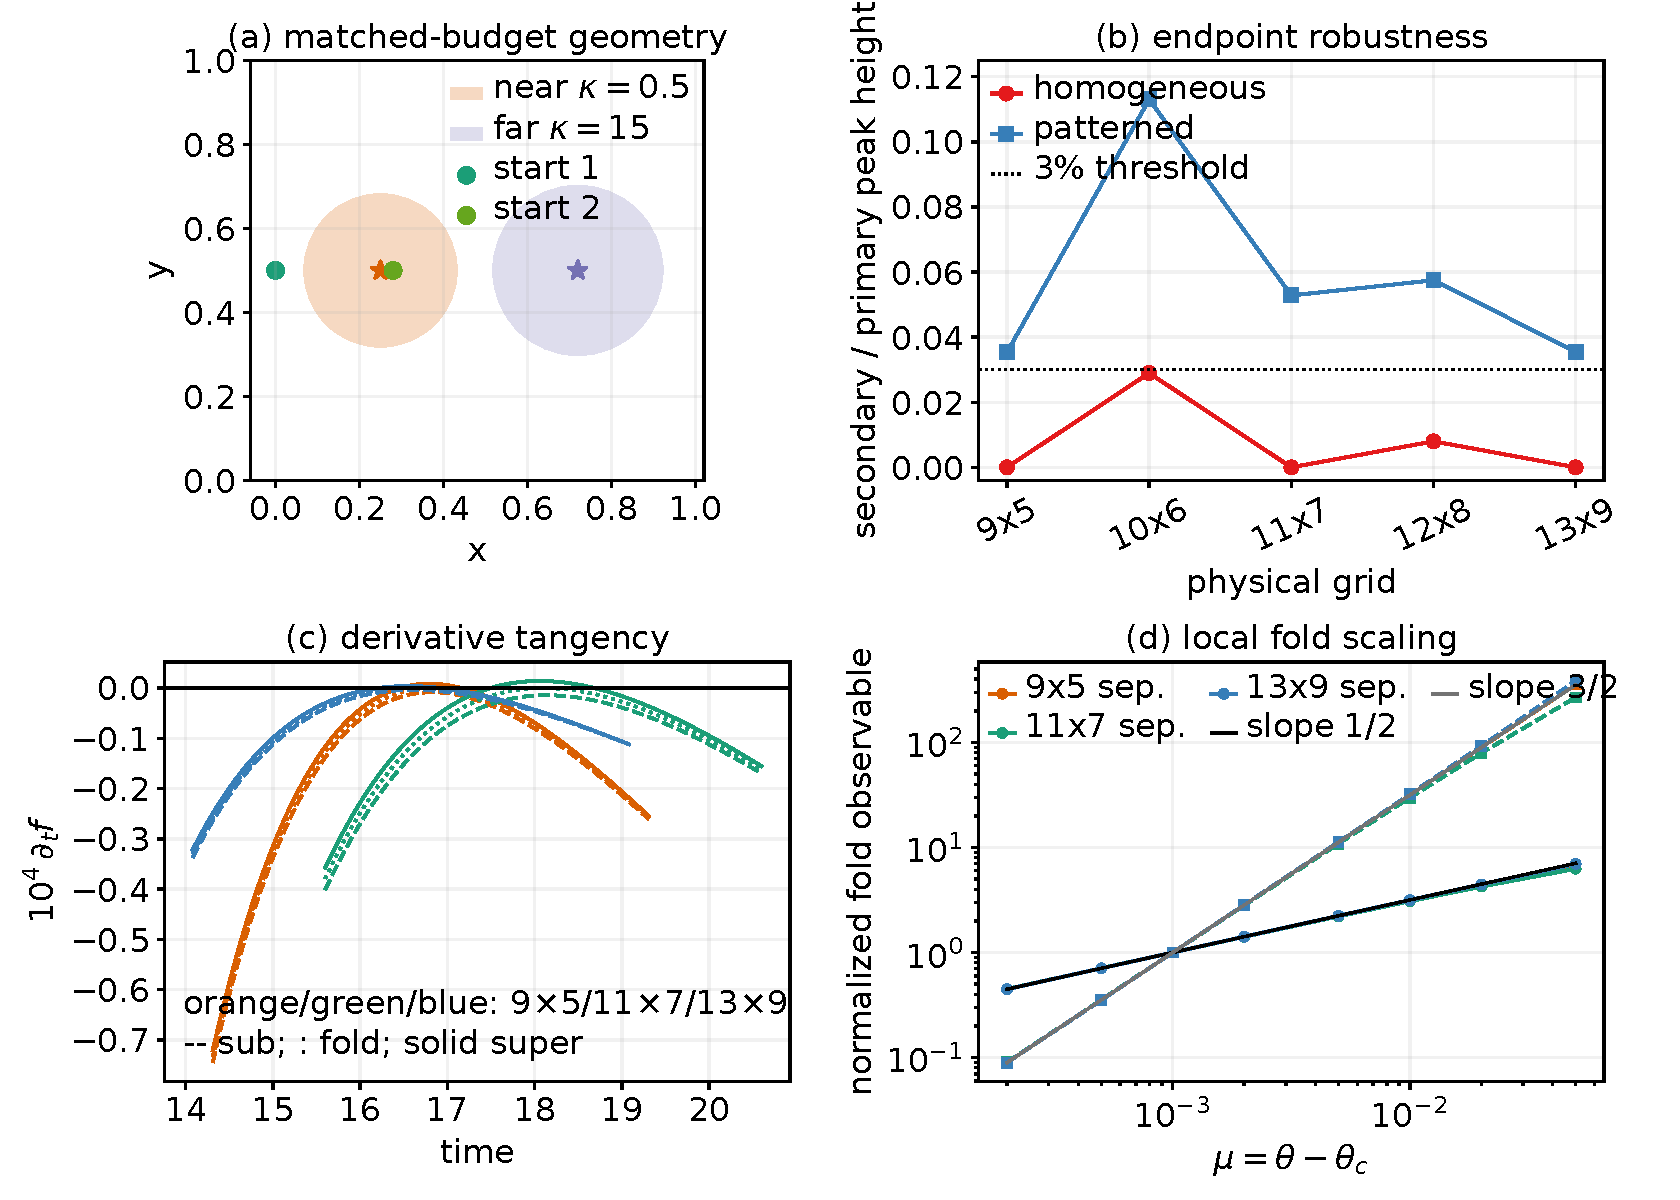
\includegraphics[width=6.65in]{finite_radius_2d_fold_validation}
\caption{\label{fig:2d-fold}
Finite-radius two-dimensional matched-budget (M2D-F) fold certificate. (a) Spatial
redistribution keeps the statewise killing sum fixed on each grid. (b) The
endpoint audit distinguishes resolved secondary peaks from reported
subthreshold ripples. (c) Analytic derivatives locate a tangency and its
two-sided continuations on three finite grids. (d) Each grid recovers square-root
separation and \(3/2\) prominence. The critical controls
\(0.275,0.014,0.256\) are explicitly nonmonotone and move under a second
budget measure; they are not estimates of a continuum fold.}
\end{figure*}

Figure~\ref{fig:2d-fold} collects the fixed-budget construction, the
endpoint morphology audit, the derivative-located folds, and their independent
normal-form scaling.

The two intervening grids are consistent with that caution. On
\(12\times8\), a nondegenerate continuation root lies at
\((t_c,\theta_c)=(18.26877,-0.06158)\), outside the physical path. On
\(10\times6\), a curvature scan over \(\theta\in[-0.2,0.1]\),
\(t\in[0.01,40]\) and four bounded least-squares starts (bounds
\(t\in[8,25]\), \(\theta\in[-0.2,0]\))
find no fold, with all starts reaching the same positive near miss
\(f_t=3.8721\times10^{-6}\). This bounded search does not cover the
interval \(\theta\approx0.25\)--\(0.28\) in which two of the three located
folds sit; it is a bounded diagnostic, not evidence of absence. Detailed endpoint roots, budget
quadrature, even-grid scans, and morphology settings are provided in the
Supplemental Material \cite{supplementalMaterial}.


\section{Continuum bridge: theory, refinement, and off-lattice validation}
\label{sec:bridge}

The finite-generator certificates of Sec.~\ref{sec:fold-results} deliberately
stopped short of any continuum claim. This section closes that gap in three
steps: an exact transfer theory specifying what discrete-to-continuum fold
inheritance requires; a cell-averaged, successively refined lattice family
that removes the two discretization pathologies of the original grids; and a
lattice-free stochastic realization of the continuum model. The combined
result is sharper than an extrapolated critical value: the physical
matched-budget path carries \emph{no} interior fold in the continuum limit,
and the fold responsible for the finite-grid observations sits outside the
physical path, extrapolating to the admissibility edge of the
redistribution family where the far-channel rate vanishes.

\subsection{Exact transfer statements}
\label{sec:bridge-theory}

Write \(F_h(t,\theta)=f_h(t,\theta)\) for the level-\(h\)
reaction density and \(F\) for a candidate continuum limit on a compact
rectangle \(N=[t_1,t_2]\times[\theta_1,\theta_2]\) with \(t_1>0\).

\paragraph{Jet convergence from sectorial resolvent convergence.}
Let \(A_h(\theta)=L_h-\operatorname{diag}k_{h,\theta}\) be the killed
generators, with
\(f_h(t,\theta)=\langle k_{h,\theta},\e^{A_h(\theta)t}p_h\rangle\), and let
\(A(\theta)\) be the continuum killed operator. Assume:
(H1) the family \(\{A_h(\theta)\}\) is uniformly sectorial---there are
\(M\ge1\), \(\omega_0\in\mathbb R\), \(\delta\in(0,\pi/2)\), independent of
\(h\) and \(\theta\), with \(\|(z-A_h(\theta))^{-1}\|\le M/|z-\omega_0|\) for
\(|\arg(z-\omega_0)|<\tfrac\pi2+\delta\);
(H1$'$) \(A(\theta)\) is sectorial on the same sector with the analogous
bound, uniformly in \(\theta\); the continuum family is affine along the
same path [Eq.~\eqref{eq:2d-budget-path}], \(A(\theta)=A(0)-\theta\,(k_{\mathrm{pat}}-\bar k)\) acting by
multiplication, with \(\theta\)-differentiable resolvent; the pairing
\(\langle k_\theta,\cdot\,\rangle\) with \(p\) is well defined uniformly in
\(\theta\); and \(f(t,\theta)=\langle k_\theta,\e^{A(\theta)t}p\rangle\)
admits the analytic-semigroup representation below, so that
\(\partial_\theta\partial_t^jf\) has the same two-term Dunford form as its
discrete counterpart. Fix \(\delta'\in(0,\delta)\), \(\rho>0\), and the
\emph{unbounded} sectorial contour
\(\Gamma=\{\omega_0+r\e^{\pm i(\pi/2+\delta')}:r\ge\rho\}\cup
\{\omega_0+\rho\e^{i\varphi}:|\varphi|\le\tfrac\pi2+\delta'\}\),
oriented from the lower ray to the upper ray (counterclockwise about the
spectrum). For \(t\ge t_1>0\) the Dunford representation
\[
\partial_t^jf_h(t,\theta)
=\frac1{2\pi i}\int_\Gamma z^j\e^{zt}\,
\langle k_{h,\theta},(z-A_h(\theta))^{-1}p_h\rangle\,\dd z,
\qquad j\le3,
\]
holds exactly for every \(h\) (and, by (H1$'$), for the continuum pair).
Define the scalar contour defects
\[
\eta_h=\sup_{\theta}\sup_{z\in\Gamma}
\big|\langle k_{h,\theta},(z-A_h(\theta))^{-1}p_h\rangle
-\langle k_{\theta},(z-A(\theta))^{-1}p\rangle\big|,
\]
and, using
\(\partial_\theta(z-A_h)^{-1}=-(z-A_h)^{-1}
\operatorname{diag}(k_{h,\mathrm{pat}}-\bar k_h)(z-A_h)^{-1}\)
(the path is affine,
\(A_h(\theta)=A_h(0)-\theta\operatorname{diag}(k_{h,\mathrm{pat}}-\bar k_h)\)),
the mixed defect \(\eta_h'\) as the same supremum for the two-term derivative
form
\(\langle k_{h,\mathrm{pat}}-\bar k_h,(z-A_h)^{-1}p_h\rangle
-\langle k_{h,\theta},(z-A_h)^{-1}
\operatorname{diag}(k_{h,\mathrm{pat}}-\bar k_h)(z-A_h)^{-1}p_h\rangle\)
against its continuum counterpart. Then, for \(j\le3\), \(l\in\{0,1\}\),
\(j+l\le3\),
\[
\sup_N\big|\partial_\theta^l\partial_t^j(f_h-f)\big|
\;\le\;C_\Gamma^{(j)}(t_1,t_2)\,\big(\eta_h+l\,\eta_h'\big),
\qquad
C_\Gamma^{(j)}
=\frac1{2\pi}\int_\Gamma\max(1,|z|)^{j}\,
\max\!\big(\e^{t_1\operatorname{Re}z},\e^{t_2\operatorname{Re}z}\big)
\,|\dd z|,
\]
finite because on the rays
\(\operatorname{Re}z=\omega_0-r\sin\delta'\), so the integrand decays like
\(r^{j}\e^{-t_1r\sin\delta'}\); the constant grows like
\(t_1^{-(j+1)}\) as \(t_1\downarrow0\), which is why the strictly positive
window is load-bearing. Hypotheses (H1), (H1$'$) and the decay of
\(\eta_h,\eta_h'\) are \emph{not} proved here for the upwind or
exponentially fitted schemes; they are the precise analytic content that the
observed ladder rates instantiate numerically.

\paragraph{Quantitative fold transfer.}
Let \(F,F_h\) have continuous \(\partial_t^jF\) (\(j\le3\)) and
\(\partial_\theta\partial_t^jF\) (\(j\le2\)) on \(N\). Assume \(F\) has an
interior fold at \(q_*=(t_*,\theta_*)\):
\(F_t(q_*)=F_{tt}(q_*)=0\), with margins
\(|F_{ttt}|\ge\mu_3>0\) and \(|F_{t\theta}|\ge\mu_\theta>0\) on \(N\).
Let \(\Lambda\) bound the sup norms
\(\|F_{t\theta}\|_N,\|F_{ttt}\|_N,\|F_{tt\theta}\|_N\), and let \(\omega\)
(part of the data) be a common nondecreasing modulus of continuity for
these three functions on \(N\); write
\(\hat\omega(r)=\max\big(\omega(r),\sqrt2\,\Lambda r\big)\) for the
augmented modulus that also controls the \(F_{tt}\) entry. Define
\[
\varepsilon_h=\max_{j=1,2}\|\partial_t^j(F_h-F)\|_{N},
\quad
\varepsilon_h'=\max\Big(\|\partial_t^3(F_h-F)\|_{N},
\max_{j\in\{1,2\}}\|\partial_\theta\partial_t^j(F_h-F)\|_{N}\Big),
\quad
\bar\varepsilon_h=\max(\varepsilon_h,\varepsilon_h').
\]
This is the \(C^3\)-versus-\(C^2\) gap: two time derivatives control the
location of the critical pair, and the third controls its nondegeneracy.
Let \(H=(F_t,F_{tt})\) with Jacobian
\(J=\begin{pmatrix}F_{tt}&F_{t\theta}\\F_{ttt}&F_{tt\theta}\end{pmatrix}\),
so \(\det J(q_*)=-F_{t\theta}(q_*)F_{ttt}(q_*)\) and
\[
\sigma:=1/\|J(q_*)^{-1}\|\;\ge\;
\frac{\mu_3\mu_\theta}{\sqrt{\mu_\theta^2+2\Lambda^2}}\,>0 .
\]
Let \(r_0=\min\big(r_\omega,\operatorname{dist}(q_*,\partial N)\big)\),
where \(r_\omega\) is any radius with \(\hat\omega(r_\omega)\le\sigma/16\)
(in particular \(r_\omega\le\sigma/(16\sqrt2\Lambda)\); so \(r_0\) is
determined by \((\mu_3,\mu_\theta,\Lambda,\omega)\) and the
position of \(q_*\) in \(N\)), and set
\[
\delta_0=\min\Big(\frac{\sigma}{32},\ \frac{\mu_3}{2},\
\frac{\mu_\theta}{2},\ \frac{5\,\sigma r_0}{8\sqrt2}\Big).
\]
If \(\bar\varepsilon_h<\delta_0\), then \(F_h\) has exactly one
solution \(q_h\) of \(F_{h,t}=F_{h,tt}=0\) in \(B(q_*,r_0)\); it is a
nondegenerate fold of \(F_h\), with margins
\(|F_{h,ttt}|\ge\mu_3-\bar\varepsilon_h>0\) and
\(|F_{h,t\theta}|\ge\mu_\theta-\bar\varepsilon_h>0\) on all of \(N\); and
\[
\|q_h-q_*\|\;\le\;2\sqrt2\,\|J(q_*)^{-1}\|\,\varepsilon_h .
\]
\emph{Converse (ladder version).} Suppose each \(F_h\) has a fold
\(q_h\in N\) with \(\operatorname{dist}(q_h,\partial N)\ge d>0\) uniformly,
the margins \(|F_{h,ttt}|\ge\mu_3\), \(|F_{h,t\theta}|\ge\mu_\theta\) hold
on \(N\), the functions
\(F_{h,t\theta},F_{h,ttt},F_{h,tt\theta}\) are bounded by \(\Lambda\) with
a common nondecreasing modulus \(\omega\) uniformly in \(h\), and the jets
\(\partial_t^jF_h\) (\(j\le3\)), \(\partial_\theta\partial_t^jF_h\)
(\(j\in\{1,2\}\)) converge uniformly on \(N\) to those of \(F\). Then for all
sufficiently fine \(h\) the limit \(F\) has a nondegenerate fold \(\bar q\)
with
\[
\|\bar q-q_h\|\le
2\sqrt2\,\frac{\sqrt{\mu_\theta^2+2\Lambda^2}}{\mu_3\mu_\theta}\,
\varepsilon_h ,
\]
and \(\bar q\) is the \emph{only} fold of \(F\) in \(N\): the \(N\)-wide
margins force \(F_{ttt}\) and \(F_{t\theta}\) to keep constant signs on the
connected rectangle, so \(F_t(\cdot,\theta)\) has a one-signed extremum
with value zero at any fold and strict monotonicity of \(F_t\) in
\(\theta\) excludes a second fold at any other \(\theta\). The proof \cite{supplementalMaterial} is a simplified-Newton contraction
seeded at the fold; no
Lipschitz control of the defect \(F_h-F\) is required.

\paragraph{Remark (a posteriori interpretation).}
Three statements of decreasing strength organize how the ladder is read.
(R1) \emph{Rigorous-conditional:} if the jets of \(F_h\) converge uniformly
on \(N\) to some \(F\) and the discrete folds, margins, and interior
distances satisfy the converse hypotheses uniformly along the ladder, then
\(F\) has a nondegenerate fold and every located discrete fold lies within
\(2\sqrt2\,\sqrt{\mu_\theta^2+2\Lambda^2}\,(\mu_3\mu_\theta)^{-1}
\varepsilon_h\) of it.
(R2) \emph{Falsification bound:} if two discretizations both satisfy the
transfer hypotheses toward the same limit and each located fold is the
unique one of the theorem's ball (both schemes track the same fold branch),
their located critical controls obey
\(|\theta_c^{(1)}(h)-\theta_c^{(2)}(h)|
\le2\sqrt2\,\|J(q_*)^{-1}\|(\varepsilon_h^{(1)}+\varepsilon_h^{(2)})\);
a large cross-scheme gap therefore falsifies joint convergence at the
claimed rates, while a small gap is necessary but not sufficient---error
components shared by both schemes (the cell-averaged masks and the budget
rule are common to both) cancel to leading order in the gap and are not
tested by it.
(R3) \emph{Error estimate under an asymptotic-regime assumption:} if the
level-to-level jet increments
\(d_k=\max_{j\le2}\|\partial_t^j(F_{h_{k+1}}-F_{h_k})\|_N\)
obey the geometric domination \(d_{m+1}\le\varrho\,d_m\) for \emph{all}
\(m\ge k\) with a fixed \(\varrho<1\)---the observed level ratios certify
this only on the computed levels, so \(\varrho\) should dominate, not
average, them, and the extension to uncomputed levels is an assumption---
then the telescoping bound
\(\tilde\varepsilon_{h_k}:=\max_{j\le2}\|\partial_t^j(F_{h_k}-F^{\rm lad}_\infty)\|_N
\le d_k/(1-\varrho)\)
controls the distance to the ladder's own jet limit \(F^{\rm lad}_\infty\);
its identification
with the continuum \(F\) is exactly the (H1)/(H1$'$) content. Richardson
extrapolants of \(\theta_c(h)\) are reported as estimates only: no
convergence rate is claimed for them unless the fitted leading coefficient
is nonzero, the observed order is stable across consecutive level triples,
and a strengthened remainder \(O(h^{p+s})\), \(s>0\), is assumed. The
cross-scheme gap of the two extrapolants is reported alongside them as a
conservative uncertainty indicator.

\subsection{Cell-averaged refined family}
\label{sec:refined-family}

The refined family keeps every physical parameter of
Sec.~\ref{sec:2d-fold-continuation} (transport, starts, contact radius,
patch geometry and rates, matched budget) and changes only the
discretization, removing its two known pathologies. First, the binary
masks are replaced by cell averages: for every product state the fraction
of its four-dimensional product cell inside the killing region
\(\{|x_1-x_2|<a\}\cap\{C_{1/2}\in\text{patch}\}\) is computed by tensorized
midpoint subsampling with four points per axis per particle cell
(\(4^4=256\) subsamples per product cell), so the killing field varies
smoothly as the grid moves across patch boundaries instead of aliasing.
Second, the grids are square-celled, \(n\times n\) nodes with
\(h=1/(n-1)\) per axis, so no aspect anisotropy enters the ladder. The
budget is matched by tensor-product boundary control-volume (trapezoidal)
weights, the per-grid homogeneous rate is recomputed so that the weighted
killing sum is \(\theta\)-invariant to \(2\times10^{-12}\) relative
(verified at both endpoints), and the per-grid budget converges to the
continuum tube integral (absolute gap \(7.3\times10^{-3}\) at \(n=9\),
\(3.6\times10^{-3}\) at \(n=13\), \(5.8\times10^{-4}\) at \(n=17\),
and bounded by \(2.0\times10^{-3}\) with alternating sign at every finer
level). Two transport
discretizations are run over the same ladder: the upwind rates of
Sec.~\ref{sec:2d-fold-continuation} and Scharfetter--Gummel exponential
fitting \cite{scharfetterGummel1969}, with per-edge P\'eclet number
\(\mathrm{Pe}=v_{\rm edge}h/D\) and
rates \((D/h^2)\,\mathrm{Pe}/(1-\e^{-\mathrm{Pe}})\) forward,
\((D/h^2)\,\mathrm{Pe}/(\e^{\mathrm{Pe}}-1)\) backward, which are positive
for all \(\mathrm{Pe}\) and reduce to central differencing as
\(\mathrm{Pe}\to0\). Folds are located exactly as before (augmented
sensitivities, analytic Jacobian, tolerance \(10^{-11}\); first-derivative
residuals below \(3.5\times10^{-13}\) and second-derivative residuals below
\(2.5\times10^{-12}\) at every accepted root).

\begin{table}[!t]
\caption{\label{tab:ladder}
Cell-averaged square-cell refinement ladder: located fold coordinates for
the two transport discretizations (upwind, UW; Scharfetter--Gummel, SG).
Every accepted root has normalized residuals at most
\(2.4\times10^{-12}\) and nondegenerate normalized margins
\cite{supplementalMaterial}. All folds from
\(n=17\) on lie outside the physical path \(\theta\in[0,1]\); the
pre-asymptotic levels \(n\le13\) are shown for completeness (the UW solver
locks onto a different root branch with \(t_c\approx10.5\), and the
\(n=9\) SG root at \(\theta_c=0.215\) is a residual coarse-cell root that
does not survive refinement).}
\begin{ruledtabular}
\begin{tabular}{rrrrr}
\(n\) & \(\theta_c^{\rm UW}\) & \(\theta_c^{\rm SG}\) &
\(t_c^{\rm UW}\) & \(t_c^{\rm SG}\)\\
\hline
9  & \(-0.1837\) & \(0.2148\)  & 10.387 & 18.607\\
13 & \(-0.1758\) & \(-0.1178\) & 10.578 & 19.327\\
17 & \(-0.0431\) & \(-0.1386\) & 17.952 & 18.293\\
21 & \(-0.1000\) & \(-0.1458\) & 18.273 & 17.796\\
25 & \(-0.1181\) & \(-0.1507\) & 18.301 & 17.442\\
29 & \(-0.1297\) & \(-0.1553\) & 18.228 & 16.977\\
33 & \(-0.1370\) & \(-0.1578\) & 18.174 & 16.811\\
\end{tabular}
\end{ruledtabular}
\end{table}


\begin{figure*}[!t]
\centering
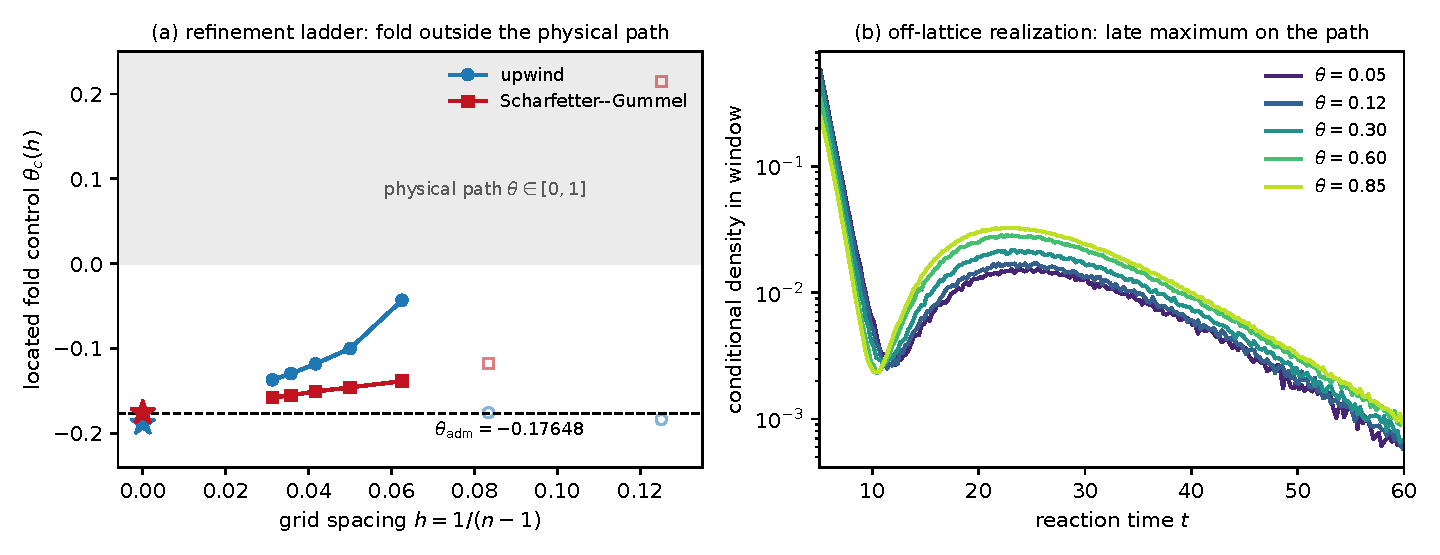
\includegraphics[width=6.6in]{encounter_continuum_bridge}
\caption{\label{fig:bridge}
Continuum bridge. (a) Located fold control \(\theta_c(h)\) for the
cell-averaged square-cell ladder under both transport discretizations
(filled markers: same-branch levels \(n\ge17\); open markers: the
pre-asymptotic levels \(n\le13\) discussed in the text). Every same-branch
root lies below the physical path (shaded); the stars at \(h=0\) are the
first-order Richardson estimates, which sit at the admissibility edge
\(\theta_{\rm adm}\) [Eq.~\eqref{eq:theta-adm}] (dashed) within their
uncertainty. (b) Off-lattice reaction-time densities
(\(2\times10^7\) walkers per control, conditioned on the window
\(t\in[5,60]\)): the valley--late-maximum structure is present at every
sampled control and strengthens monotonically with \(\theta\).}
\end{figure*}

Table~\ref{tab:ladder} and Fig.~\ref{fig:bridge}(a) report the ladder. Three features are decisive.
First, from \(n=17\) on, \emph{both} discretizations place the fold at
negative control, outside the physical path \(\theta\in[0,1]\), with
nondegenerate normalized margins throughout. Second, the two sequences
approach each other as the grid refines: the cross-discretization gap in
\(\theta_c\) falls from \(0.095\) at \(n=17\) to \(0.046\) at \(n=21\),
\(0.033\) at \(n=25\), \(0.026\) at \(n=29\), and \(0.021\) at
\(n=33\). Third, the coarse levels
\(n\le13\) are pre-asymptotic: the upwind solver locks onto a different
root branch (fold times near \(t\approx10.5\) instead of
\(t\approx17\)--\(18\)), and the \(n=9\) Scharfetter--Gummel fold is the
single physical-interval exception (\(\theta_c=0.215\)) that disappears
under its own refinement; at \(n=9\) a further \(7.1\%\) of the initial
mass lies inside the contact tube (exactly zero at every finer level),
compounding the coarse-cell error at that single level.
Restricting to the same-branch levels \(n\ge17\), first-order Richardson
extrapolation on the finest level pair gives \(\theta_*\approx-0.19\)
(upwind) and \(\theta_*\approx-0.18\) (Scharfetter--Gummel); the observed
order is not yet stable across level triples, so, per the a posteriori
remark of Sec.~\ref{sec:bridge-theory}, these extrapolants are reported as
estimates with the cross-scheme gap as a conservative uncertainty
indicator, and no convergence rate is claimed for them. They are to be compared with the
admissibility edge of the matched-budget family: the path rate
[Eq.~\eqref{eq:2d-budget-path}] on the far
patch, \((1-\theta)\bar\kappa+15\,\theta\), first becomes negative at
\begin{equation}
\theta_{\rm adm}
=-\frac{\bar\kappa}{15-\bar\kappa}
=-0.17648\ldots,
\qquad \bar\kappa=2.2501572\ldots,
\label{eq:theta-adm}
\end{equation}
so the extrapolated fold sits at (or within the extrapolation uncertainty
of) the boundary at which the far channel shuts off entirely. What the
ladder does establish, at every level \(n\ge17\) and for both
discretizations, is that the located fold lies outside the physical path:
the three binary-mask folds of Sec.~\ref{sec:2d-fold-continuation} do not
persist under refinement, and their nonmonotone, budget-measure-sensitive
critical controls are explained as artifacts of the coarse binary-mask,
equal-weight discretization they were computed with.

\subsection{Off-lattice stochastic validation}
\label{sec:offlattice}

A lattice-free realization removes the remaining dependence on any grid.
Two particles obey the continuum model directly
(Euler--Maruyama, \(\dd X_i=v_i\,\dd t+\sqrt{2D_i}\,\dd W\),
transverse Ornstein--Uhlenbeck restoring drift, reflecting walls,
\(\dd t=2\times10^{-4}\)), and while \(|X_1-X_2|<a\) the pair is killed at
rate \(\kappa_\theta(C_{1/2})\) with per-step probability
\(1-\e^{-\kappa\,\dd t}\). The continuum homogeneous matched rate
\(\bar\kappa=2.2501572\) reproduces the exact tube-integral reference to
all printed digits and is cross-checked by a \(10^8\)-sample Monte-Carlo
volume estimate to \(0.12\%\). Consistency checks: zero kills at
\(\kappa=0\) over \(2.5\times10^7\) contact steps; per-step kill
probabilities within \([0,1]\); halving \(\dd t\) at \(2\times10^5\) walkers
(\(\theta=0.12\) and \(0.60\)) changes the windowed histograms by amounts
consistent with pure counting noise (per-bin \(|z|\) averaging
\(0.72\)--\(0.75\), \(\max|z|\le3.1\) over \(50\)--\(55\) bins).

With \(2\times10^7\) walkers per control value, the reaction-time density
shows a significant late second maximum throughout the sampled physical
path: at \(\theta=0.05,0.12,0.30\) the smoothed
histograms give second maxima at \(t=24.6,23.4,22.9\) with Poisson
significances \(12.6\sigma,14.0\sigma,18.7\sigma\) and
\(0.8\)--\(1.8\times10^5\) events in the diagnostic window
\(t\in[10,30]\); at \(\theta=0.60\) the second maximum reaches
\(31.8\sigma\) with \(5.1\times10^5\) window events, and at
\(\theta=0.85\) it reaches \(52.3\sigma\) at \(t=22.6\) with
\(1.4\times10^6\) window events. The late-peak
prominence \emph{increases} monotonically with \(\theta\) over the sampled
range: patterned redistribution strengthens the far-channel peak, and
nowhere on the sampled physical path does the maximum--minimum pair
annihilate. Figure~\ref{fig:bridge}(b) shows the windowed densities. The off-lattice
model therefore agrees with the refined ladder
on both counts: the physical family is uniformly two-peaked, and the fold
that the finite-grid family kept locating inside \([0,1]\) is not a
continuum feature of the physical path.

\subsection{Interpretation}
\label{sec:bridge-interpretation}

Three independent lines---the transfer theory, the two-discretization
refinement ladder, and the lattice-free realization---assemble into one
statement: for this geometry the matched-budget redistribution path
possesses no interior continuum fold; the organizing fold of the
finite-window morphology lies just outside the path, at negative control
near \(\theta_{\rm adm}\) [Eq.~\eqref{eq:theta-adm}], where the admissible
family terminates because the far-patch rate reaches zero. The finite-generator certificates of
Sec.~\ref{sec:fold-results} remain exactly what they were declared to be:
correct statements about their own generators, whose critical controls are
now shown---rather than merely suspected---not to survive refinement. The
practical lesson for reaction-field design is correspondingly sharpened:
on this path, spatial redistribution at fixed budget \emph{tunes} the
relative weight of the two arrival-time scales but cannot merge them; the
merger happens only at the edge of admissibility, in the limit of complete
far-channel shutdown.

\section{Discussion and scope}
\label{sec:discussion}

The finite-model calculation separates three questions. Transport determines
which temporal scales are available. The initial and reaction observables
determine the signs and amplitudes of their spectral residues. Finally, a
declared feasible reaction-field perturbation determines whether the
critical-point equation can be crossed. Patch count alone addresses none of
these questions: a support-rank-one counterexample can already be bimodal,
whereas a residue sequence with three sign changes need not have three
positive derivative roots.

The Green reduction and sensitivity calculus play complementary roles.
\(\Gres(s)\) reduces transport to the reaction support, while
Eqs.~\eqref{eq:modality-susceptibility}--\eqref{eq:optimal-redistribution}
operate directly on the time-domain fold equation. A killed pole can be dark
or cancel from a selected observable, and a density fold is not a spectral
exceptional point. The spectral sign count is therefore used only to
falsify an impossible finite reversible mode count, never to replace direct
time-derivative root calculations.

The finite encounter CTMC confirms the derivative chain but has a very small
minority channel. The M2D-F result more directly tests spatial redistribution
at a fixed per-grid budget, yet its grid and budget-measure sensitivity
prevents a continuum interpretation. The supporting Supplemental Material
shows additionally that spatial patterning can promote an existing
subthreshold maximum across an operational resolution threshold in a separate
endpoint family, but is not necessary for bimodality; a uniformly reactive
finite model provides a counterexample \cite{supplementalMaterial}. It also
records catalytic-coordinate sensitivity and underresolved three-patch
finite-grid examples. Those controls restrict causal language rather than
broaden the principal claim.

The continuum bridge is settled in Sec.~\ref{sec:bridge}. The
\(C^3\)-versus-\(C^2\) distinction that governs fold transfer is made
exact by the transfer theorem there, and the cell-averaged,
two-discretization refinement it prescribes returns a negative verdict for
this geometry: no interior fold survives on the physical path, and the
finite-grid critical controls are artifacts of the coarse binary-mask
discretization (Secs.~\ref{sec:refined-family} and \ref{sec:offlattice}).

Other limits remain explicit. The projected optimum is local and ignores
finite-amplitude nonnegativity, box constraints, binary supports, and
nonsmooth patch motion. The Green identity is a right-half-plane
volume-reaction statement under its operator hypotheses; an unqualified
Robin trace analogue and continuum meromorphic continuation are not supplied.
The original 2D grids use upwind transport and binary masks; the
cell-averaged ladder and Brownian realization of Sec.~\ref{sec:bridge}
quantify exactly what those choices affected. The sectorial and jet
hypotheses of Sec.~\ref{sec:bridge-theory} are instantiated numerically
rather than proved for these schemes, the ladder extrapolants carry no
claimed convergence rate, and the off-lattice family samples five control
values. The chosen discrete state-sum budget
does not equalize pathwise hazards, splitting probabilities, or mean
lifetimes. Capacity and GIG calculations in the Supplemental Material are
calibration and screening layers, not centre-patterned modality theorems.

\section{Conclusions}
\label{sec:conclusions}

For a declared finite encounter generator, the observable spectral residues
give a necessary sign-variation gate, and the Fr\'echet--Duhamel derivative
gives the exact local response of the critical-point equation to the killing
field. Projection onto a budget tangent space then identifies the steepest
unit feasible redistribution in a chosen metric. These statements link
transport, reaction observability, and admissible control without equating
the number of catalytic patches with the number of modes.

Two numerical certificates exercise the calculus. A finite two-reactant CTMC
has a nondegenerate density fold with direct residual and transversality
checks and the expected continuation exponents. A separate finite-radius M2D-F
path has analogous folds on three finite grids under an exactly fixed
per-grid killing sum. Their critical controls are nonmonotone and
budget-measure sensitive, and the continuum study of Sec.~\ref{sec:bridge}
explains why: under cell-averaged refinement with two independent transport
discretizations the located fold leaves the physical path, and the
lattice-free realization confirms a two-peaked density at every sampled
control.
The finite-generator certificates therefore stand as declared, and the
continuum statement this article adds is a negative one with a sharp
boundary mechanism: at fixed budget, redistribution on this path tunes but
cannot merge the two arrival-time scales; merger occurs only at the
admissibility edge of complete far-channel shutdown.

\section*{Data Availability}

The source code, numerical tables, vector figures, and machine-readable
provenance manifests that reproduce every reported number are available from
the author upon reasonable request, and will accompany the published article
as a public, versioned archive.

\bibliography{references}

\end{document}
